\documentclass[10pt,landscape]{article}

%
\usepackage[T1]{fontenc}

\usepackage{multicol}
\usepackage{calc}
\usepackage{ifthen}
\usepackage[landscape]{geometry}
\usepackage{hyperref}
\usepackage{graphicx}
\usepackage{amsmath,amssymb}
\usepackage[noend]{algorithm2e}
\usepackage{float}
\usepackage{xcolor}
\usepackage{bbm}
\usepackage{placeins}
\usepackage{enumitem}
% To make this come out properly in landscape mode, do one of the following
% 1.
%  pdflatex rl_cheatsheet.tex
%
% 2.
%  latex rl_cheatsheet.tex
%  dvips -P pdf  -t landscape rl_cheatsheet.dvi
%  ps2pdf rl_cheatsheet.ps


% 2022-01
% Thomas - made changes for Stanford's CS234 2022 RL lecture

% If you're reading this, be prepared for confusion.  Making this was
% a learning experience for me, and it shows.  Much of the placement
% was hacked in; if you make it better, let me know...


% 2008-04
% Changed page margin code to use the geometry package. Also added code for
% conditional page margins, depending on paper size. Thanks to Uwe Ziegenhagen
% for the suggestions.

% 2006-08
% Made changes based on suggestions from Gene Cooperman. <gene at ccs.neu.edu>


% To Do:
% \listoffigures \listoftables
% \setcounter{secnumdepth}{0}


% This sets page margins to .5 inch if using letter paper, and to 1cm
% if using A4 paper. (This probably isn't strictly necessary.)
% If using another size paper, use default 1cm margins.
\ifthenelse{\lengthtest { \paperwidth = 11in}}
        { \geometry{top=.5in,left=.5in,right=.5in,bottom=.5in} }
        {\ifthenelse{ \lengthtest{ \paperwidth = 297mm}}
                {\geometry{top=1cm,left=1cm,right=1cm,bottom=1cm} }
                {\geometry{top=1cm,left=1cm,right=1cm,bottom=1cm} }
        }

% Turn off header and footer
\pagestyle{empty}


% Redefine section commands to use less space
\makeatletter
\renewcommand{\section}{\@startsection{section}{1}{0mm}%
                                {-1ex plus -.5ex minus -.2ex}%
                                {0.5ex plus .2ex}%x
                                {\normalfont\large\bfseries}}
\renewcommand{\subsection}{\@startsection{subsection}{2}{0mm}%
                                {-1explus -.5ex minus -.2ex}%
                                {0.5ex plus .2ex}%
                                {\normalfont\normalsize\bfseries}}
\renewcommand{\subsubsection}{\@startsection{subsubsection}{3}{0mm}%
                                {-1ex plus -.5ex minus -.2ex}%
                                {1ex plus .2ex}%
                                {\normalfont\small\bfseries}}
\makeatother

% Define BibTeX command
\def\BibTeX{{\rm B\kern-.05em{\sc i\kern-.025em b}\kern-.08em
    T\kern-.1667em\lower.7ex\hbox{E}\kern-.125emX}}

% Don't print section numbers
\setcounter{secnumdepth}{0}


\setlength{\parindent}{0pt}
\setlength{\parskip}{0pt plus 0.5ex}

\DeclareMathOperator*{\argmax}{argmax}

% -----------------------------------------------------------------------

\begin{document}

\raggedright
\footnotesize
\begin{multicols}{3}

% multicol parameters
% These lengths are set only within the two main columns
%\setlength{\columnseprule}{0.25pt}
\setlength{\premulticols}{1pt}
\setlength{\postmulticols}{1pt}
\setlength{\multicolsep}{1pt}
\setlength{\columnsep}{2pt}

\newlength{\MyLen}
\settowidth{\MyLen}{\texttt{letterpaper}/\texttt{a4paper} \ }

\begin{center}
\centering\Large{CS234 - Reinforcement Learning}\phantom{---}
\end{center}

%%\section{Agent-Environment Interface}
%\includegraphics[width=\linewidth]{./images/Agent-Environment.png}
%\textit{The agent at each step $t$ receives a representation of the environment's state $S_t \in S$ and it selects an action $A_t$. As a consequence  the agent receives a reward $R_{t + 1} \in \mathbb{R}$.}


\vspace{1mm}

A Markov Reward Process (\textbf{MRP}) is a Markov chain + rewards (everything only depends on the state $R(s_t=s)$).


The \textbf{total reward} (the \textbf{return}) is 
\vspace{-3mm}
\begin{align*}
G_t &= r_t+\gamma r_{t+1}+\gamma^2 r_{t+2}+\dots
+
\gamma^{H-1}r_{t+H-1}
=
\sum_{k = 0}^{H-1} \gamma^kr_{t + k}.
\end{align*}
\vspace{-4mm}

\textbf{Expected return}: 
\begin{align*}
V(s)&=\mathbb{E}[G_t|s_t=s]
=
R(s)+\gamma\sum_{s'\in\mathcal{S}}P(s'|s)V(s').
\end{align*}
Let a $N$-dim statespace,  $V=(V(s_1),\dots,V(s_N))\in\mathbb{R}^N$, $R,V\in\mathbb{R}^N$, and $P\in\mathbb{R}^{N\times N}$ with $P_{ij}=P(s_j|s_i)$. Then, we can write the matrix equation $V=R+\gamma PV$ and invert it $V=(I-\gamma P)^{-1}R$.  Complexity of doing matrix inverse is $O(N^3)$. Otherwise, do,  iteratively over $k$, for all $s\in S$, 
$$
V_k(s)=R(s)+\gamma\sum_{s'\in S}P(s'|s)V_{k-1}(s'),
\ \text{($O(N^2)$ complexity)}$$


%\vspace{2mm}
%\subsection{Markov Decision Process (MDP)}
A \underline{Markov Decision Process (\textbf{MDP})} is a 5-tuple $(S, A, P, R, \gamma)$ where $P$ is a transition model $P(s_{t+1}=s'|s_t=s,a_t=a)$ and $R$ is reward function $R(s,a)$ and $\gamma\in[0,1]$ is discount factor. 

 
\textbf{State-Value Function} (expected return under $\pi$ from $s$):
\begin{align*}
V^{\pi}(s) &= \mathbb{E}_\pi[G_t | s_t = s]
= \mathbb{E}_\pi[r_t+\gamma r_{t+1}+\gamma^2r_{t+2}+\dots | s_t = s].
\end{align*}

\textbf{Optimal policy}: $\pi^*=\mathop{\arg\max}\limits_\pi V^{\pi}(s)$.

\textbf{State-Action Value Function} (expected return  starting from $s$, taking action $a$, then following $\pi$):
\begin{align*}
Q^{\pi}(s,a) &= \mathbb{E}_\pi[G_t | s_t = s, a_t=a]
\\&= \mathbb{E}_\pi[r_t+\gamma r_{t+1}+\gamma^2r_{t+2}+\dots| s_t = s, a_t=a ]
\\
&=R(s,a)+\gamma\sum_{s'}P(s'|s,a)V^\pi(s')
\end{align*}

\textbf{Bellman Backup}: 
$$(BV)(s)=\mathop{\max}\limits_a (R(s,a)+\gamma\sum\limits_{s'}P(s'|s,a)V(s'))$$
\vspace{-5mm}
$$(B^\pi V)(s)=\sum\limits_{a}\pi(a|s)\left(R(s,a)+\gamma\sum\limits_{s'}P(s'|s,a)V(s')\right)$$

\underline{\textbf{Policy Evaluation$(\pi)$:}}
\begin{algorithm}[H]
 $V^\pi_0(s) \gets 0$ for all $s$ \\
 \While{$\|V^\pi_{k+1}-V^\pi_k\|>\epsilon$}{
  \ForAll{$s \in S$} {
%        \textbf{Bellman backup}: 
        $V_{k+1}^\pi(s) =(B^\pi V_k^\pi)(s)$.
%        =
%        \sum\limits_{a}\pi(a|s)\left(
%        r(s,a)+\gamma\sum\limits_{s'}p(s'|s,a)V_{k-1}^\pi(s')
%        \right)
%        $
  }
 }
\end{algorithm}

\underline{\textbf{Policy Improvement$(V^\pi)$:}}
%\begin{algorithm}[H]
% \ForAll{$s \in S$, $a\in A$} {
        $
        Q^{\pi}(s,a)  =R(s,a)+\gamma\sum_{s'}P(s'|s,a)V^\pi(s')
        \ \forall s\in S, a \in A
        $
% }
\\
% \ForAll{$s \in S$} {
        $
        \pi'(s)  =\mathop{\arg\max}\limits_a Q^{\pi}(s,a)
        \quad \forall s\in S
        $
% }
%\end{algorithm}

%\hline

\underline{\textbf{Policy Iteration:}}
\begin{algorithm}[H]
  $\pi_0(s) \gets \textrm{whatever}(A)$ for all $s$  \\
 \While{$\|\pi_{k+1}-\pi_k\|>\epsilon$}{
        $V^\pi_{k}\gets\textrm{PolicyEvaluation}(\pi_k)$ 
        \\
        $\pi_{k+1}(s) \gets\textrm{PolicyImprovement}(V^\pi_{k})$ 
 }
\end{algorithm}


\underline{\textbf{Value Iteration:}}
\begin{algorithm}[H]
  $V_0(s) \gets 0$ for all $s$ 
  \\
 \While{$\|V_{k+1}-V_k\|>\epsilon$}{
  \ForAll{$s \in S$} {
        $V_{k+1}(s) =  (BV_{k})(s)$
%        \max\limits_a \left(
%        R(s,a)+\gamma\sum\limits_{s'}
%                P(s'|s,a)V_k(s')
%                \right)$ 
  }
 }
% Get $\pi(s) = \argmax\limits_a \left(
%        R(s,a)+\gamma\sum\limits_{s'}
%                P(s'|s,a)V_{\textrm{end}}(s')
%                \right)$
\end{algorithm}
\vspace{-1mm}
These algorithms assume Markov and require knowledge of the dynamics $P$. Instead, we can do (model-free) \textbf{Monte-Carlo} (requires fully observed finite episode). It is unbiased (assumes infinite-horizon problem (so that time-invariant policy) that is always eventually stopped (at the stopping time $T$)). 





\underline{\textbf{MonteCarlo$(\pi)$}}
\begin{algorithm}[H]
$N(s)=0$, $G(s)=0$, \textcolor{blue}{$V^\pi(s)=0$} for all $s$ \\
 \For{$i=0,\dots$}{
    sample episode $(s_{i,1},a_{i,2},\dots,s_{i,T_i})$ with $a_{i,t}{\sim}\pi(s_t)$
    \\
    $G_{i,t}\gets r_{i,t}+\gamma r_{i,t+1}+\dots+\gamma^{T_i-1}r_{r_i,T_i}
   $ for all $t$
   \\
    \For{$t=1,\dots,T_i$}{
    $s\gets s_{i,t}$
    \\
    \If{$s$ visited for the \textbf{first} time in episode $i$}{
        $N(s)=N(s)+1$
        \\
        $G(s)=G(s)+G_{i,t}$
        \\
        $V^\pi(s) =G(s)/N(s)$
        \\
        \scalebox{0.9}{\textcolor{blue}{($V^\pi(s) \gets V^\pi(s) + \alpha(G_{i,t}-V^\pi(s))$
        (Incremental))}}
        \\
        \scalebox{0.9}{\textcolor{olive}{($\Delta w = \alpha (G_{i,t}-\phi(s_{i,t})^\top w)\phi(s_{i,t}) $
        \ \ (MC linear))}}
    }
    }
 }
\end{algorithm}
\vspace{-1mm}
The above is \textbf{first-visit} MC. Without the \textit{if}, it is \textbf{every-visit} MC (which is biased but consistent and has better MSE).
\\
\textcolor{orange}{\underline{Modification to get $Q^\pi$}: use $N(s,a)=N(s,a)+1$ and set $Q^\pi(s,a) = Q^\pi(s,a) + \alpha(G_{i,t}-Q^\pi(s,a))$ with $\alpha=\frac{1}{N(s,a)}$.}


\underline{\textbf{TD(0)$(\pi)$}} (instead of waiting for the full episode to finish)
\begin{algorithm}[H]
$V^\pi(s)=0$ for all $s$ \\
 \For{$i=0,\dots$}{
    sample tuple $(s_t,a_t,r_t,s_{t+1})$ with $a_{t}\sim\pi(s_t)$
    \\
    $V^\pi(s_t) \gets V^\pi(s_t) + \alpha\Big(\underbrace{(r_t+\gamma V^\pi(s_{t+1}))}_{\text{TD target \textit{(bootstrap})}}-V^\pi(s)\Big)$
        \\
        \scalebox{0.9}{\textcolor{olive}{($\Delta w = \alpha (r_t+\gamma\phi(s_{t+1})^\top w-\phi(s_t)^\top w)\phi(s_t) $
        \ \ (TD$(0)$ linear))}}
    }
\end{algorithm}

\underline{Certainty-Equivalence (\textbf{CE})} (MLE estimate for $P$ and $R$)
\begin{algorithm}[H]
 \For{$t=0,\dots$}{
    sample tuple $(s_t,a_t,r_t,s_{t+1})$ with $a_{t}\sim\pi(s_t)$
    \\
    $\hat{P}(s'|s,a) = \frac{1}{N(s,a)}\sum\limits_{r=1}^t\mathbbm{1}(s_r=s,a_r=a,s_{r+1}=s')$
    \\
    $\hat{r}(s,a) = \frac{1}{N(s,a)}\sum\limits_{\ell=1}^t\mathbbm{1}(s_\ell=s,a_\ell=a)r_\ell$
    }
\end{algorithm}







\underline{\textbf{SARSA} and \textcolor{blue}{\textbf{Q-Learning}}} with $\epsilon$-greedy policy
\begin{algorithm}[H]
$a_0\sim\pi(s_0)$ w.p. $1-\epsilon$ else $a_0\gets\text{random}(A)$
\\
Observe $(r_0,s_1)$
\\
 \For{$t=0,\dots$}{
 Take $a_{t+1}\sim\pi(s_{t+1})$, observe  $(r_{t+1}, s_{t+2})$
    \\
    $Q(s_t,a_t) \scalebox{1}{$\gets Q(s_t,a_t) + \alpha(r_t+\gamma Q(s_{t+1},a_{t+1})-Q(s_t,a_t))$}$
    \\
    \textcolor{blue}{$Q(s_t,a_t) \scalebox{1}{$\gets Q(s_t,a_t) + \alpha(r_t+\gamma \mathop{\max}\limits_{a}Q(s_{t+1},a)-Q(s_t,a_t))$}$}
    \\
    \scalebox{1}{$\pi(s)\gets\{\mathop{\arg\max}\limits_{a}Q(s,a)$ w.p. $1-\epsilon$ else $\text{random}(A)\}$}
    }
\end{algorithm}
\textbf{SARSA} (an \textit{on-policy} algorithm) uses every element of the tuple $(s_t,a_t,r_t,s_{t+1},a_{t+1})$. \textbf{Q-Learning} (\textit{off-policy}) allows learning optimum from arbitrary policies (only used for exploration) but suffers from the maximization bias. Thus, \textbf{Double Q-Learning} separates max action estimation with max value estimation: with probability 1/2, alternate between $Q_1$ and $Q_2$: for $1$, set \textcolor{blue}{$a^{*1}_{t+1}=\mathop{\arg\max}\limits_{a}Q_1(s_{t+1},a)$} and evaluate
\vspace{-3mm}
\begin{center}
\scalebox{1}{$
\textcolor{blue}{Q_1}(s_t,a_t) \gets \textcolor{blue}{Q_1}(s_t,a_t) + \alpha(r_t+\gamma \textcolor{red}{Q_2}(s_{t+1},\textcolor{blue}{a^{*1}_{t+1}})-\textcolor{blue}{Q_1}(s_t,a_t))$}
\\
    \scalebox{1}{$\pi(s)\gets\{\mathop{\arg\max}\limits_{a}(\textcolor{blue}{Q_1}+\textcolor{red}{Q_2})(s,a)$ w.p. $1-\epsilon$ else $\text{rand}(A)\}$}
\end{center}





\subsubsection{Value function approximation}
\scalebox{0.85}{$S$ and $A$ are assumed finite-dim. Define the loss $
J(w)=\mathbb{E}_\pi[(V^\pi(s)-\hat{V}^\pi(s;w))^2]$. } 
\scalebox{0.875}{Then, supervised learning: $
%J(w)=\mathbb{E}_\pi[(V^\pi(s)-\hat{V}^\pi(s;w))^2],
%\ \ 
\Delta w\mathop{=}\limits^{\textrm{SGD}}-\frac{1}{2}\alpha\left(2\mathbb{E}_\pi[V^\pi(s)-\hat{V}^\pi(s;w)]\nabla_w\hat{V}^\pi(s;w)\right)
$}
\underline{\textbf{Linear}}: \scalebox{1}{$\hat{V}(s;w)=\phi(s)^\top w\implies \nabla_w\hat{V}(s;w)=\phi(s)$. 
\phantom{$1_{1_{1_1}}$}}

\underline{\textbf{MC \textcolor{olive}{$\pi$ evaluation}}}: dataset $\{(s_t,G_t)\}_t$, use $ V^\pi(s_t)\approx G_t$

Converges to min	 $\textrm{MSVE}_\mu(w)=\sum\limits_s\mu(s)(V^\pi(s)-\hat{V}^\pi(s;w))^2$


\underline{\textbf{TD \textcolor{olive}{$\pi$ evaluation}}}: dataset $\{(s_t,r_t+\gamma\hat{V}^\pi(s_{t+1};w))\}_t$%\approx \{(s_t,V^\pi(s_t))\}_t$

\scalebox{1}{Let $d(s)$ stationary distribution s.t. $d(s')=\sum\limits_s\sum\limits_a\pi(a|s)p(s'|s,a)d(s)$}

\scalebox{0.95}{Converges to min $\textrm{MSVE}_d(w_{TD})\leq\frac{1}{1-\gamma}\min\limits_w
\sum\limits_sd(s)(V^\pi(s)-\hat{V}^\pi(s;w))^2$}

\underline{\textbf{SARSA},  \textcolor{blue}{\textbf{Q-Learning}}, and \textcolor{orange}{MC control}}: do the same for $Q$:
\begin{align*}
    \Delta w&=
    \alpha(r+\gamma \hat{Q}(s',a';w)-\hat{Q}(s,a;w))\nabla_w \hat{Q}(s,a;w)
    \\
    \textcolor{blue}{\Delta w}&=
    \textcolor{blue}{\alpha(r+\gamma \max\limits_{a'}\hat{Q}(s',a';w)-\hat{Q}(s,a;w))\nabla_w \hat{Q}(s,a;w)}
    \\
    \textcolor{orange}{\Delta w}&\textcolor{orange}{=
    \alpha(G_t-\hat{Q}(s_t,a_t;w))\nabla_w \hat{Q}(s_t,a_t;w)}
\end{align*}
Instability: (1) function approx (2) bootstrapping (3) off-policy

\vspace{1mm}

\underline{\textbf{Deep Q-Learning}}: (1) correlated samples (2) non-stationary \scalebox{1}{targets are addressed via (a) \textcolor{olive}{experience replay} (b) \textcolor{blue}{fixed Q-targets}  
}
\begin{algorithm}[H]
 \For{$t=0,\dots$}{
 Sample $a_t$ given $\epsilon$-greedy policy from $\hat{Q}(s_t,a;w)$
 \\
 Observe $(r_t,s_{t+1})$
 \\
 \textcolor{olive}{Store $(s_t,a_t,r_t,s_{t+1})$ in replay buffer $D$}
 \\
 \textcolor{olive}{Sample minibatch from $D$}
 \\
 \For{\textcolor{olive}{tuple in minibatch}}{
 \scalebox{1}{$\Delta w=\alpha(r+\gamma \max\limits_{a'}\textcolor{blue}{\hat{Q}(}s',a';\textcolor{blue}{w^-)}-\hat{Q}(s,a;w))\nabla \hat{Q}(s,a;w)$}
%\\
%$
%\textcolor{blue}{Q_1}(s_t,a_t) \gets \textcolor{blue}{Q_1}(s_t,a_t) + \alpha(r_t+\gamma \textcolor{red}{Q_2}(s_{t+1},\textcolor{blue}{a^{*1}_{t+1}})-\textcolor{blue}{Q_1}(s_t,a_t))$
 	}
 \textcolor{blue}{\If{sometimes}{$w^-\gets w$}}
 }
\end{algorithm}

\textbf{Double DQN} even better
$$\Delta w=\alpha(r+\gamma \hat{Q}(s',\mathop{\arg\max}\limits_{a'}\hat{Q}(s'a';w);w^-)-\hat{Q}(sa;w))\nabla \hat{Q}(sa;w)$$

\textbf{Prioritized Experience Replay}: select $i$th tuple such that 
$$p_i=|
r+\gamma\max_{a'}Q(s',a';w^-)-Q(s,a;w)
|
\ \ \text{$\forall i$th tuple in $D$}$$
\scalebox{1}{then choose $i$th tuple $(s,a,r,s')\in D$ for $\Delta w$ update with $\max\limits_ip_i$.} 
\scalebox{1}{Else, select with stochastic
prioritization, where \smash{$P(i)=p_i^\beta/\left(\sum_j p_j^\beta\right)$}.}

\vspace{1mm}

\scalebox{1}{\textbf{Advantage Function} (Dueling DQN) Features to represent $V$ well} may be
different than those to compare $Q(s,a_1)$ vs $Q(s,a_2)$.	
$$\text{Define }\quad 
A^\pi(s,a)=
Q^\pi(s,a)-
V^\pi(s). \quad \text{Then, to get $\hat{Q}$:}
$$
\begin{align*}
\hat{Q}(s,a;w)&=\hat{V}(s;w)+\Big(\hat{A}(s,a;w)-\max\limits_{a'}\hat{A}(s,a';w)\Big)
\\[-2mm]
\hat{Q}(s,a;w)&=\hat{V}(s;w)+\Big(\hat{A}(s,a;w)-\frac{1}{A}\sum_{a'}\hat{A}(s,a';w)\Big)
\end{align*}


\newpage
\textbf{Summary}:
\begin{itemize}[leftmargin=4.5mm]
\item \textbf{Model-based RL} 
\begin{itemize}[leftmargin=2.5mm]
\item[+] \textit{easy} to learn a model (supervised learning)
\item[+] learns \textit{all there is to know} from the data
\item[-] uses compute \& capacity on irrelevant details
\item[-] computing $\pi$ (planning) non-trivial / expensive
\end{itemize}
\item \textbf{Value-based RL}
\begin{itemize}[leftmargin=2.5mm]
\item[+] easy to get policy (e.g., $\pi(a|s) = \mathbbm{1}(a = \arg\max Q(s, a))$)
\item[+] close to true objective
\item[+] fairly well-understood, good algorithms exist
\item[-] still not the true objective (may focus capacity on irrelevant details, small value error can lead to larger policy error)
\end{itemize}
\item \textbf{Policy-based RL}
\begin{itemize}[leftmargin=2.5mm]
\item[+] true objective
\item[+] easy to extend to high-dim or continuous $A$
\item[+] can learn stochastic policies
\item[+] policies can be simple compared to values / models
\item[-] local minima
\item[-] does not always generalise well
%\item[-] does not necessarily extract all useful information from data
\end{itemize}
\end{itemize}

%\begin{figure}[!htb]
%\FloatBarrier
%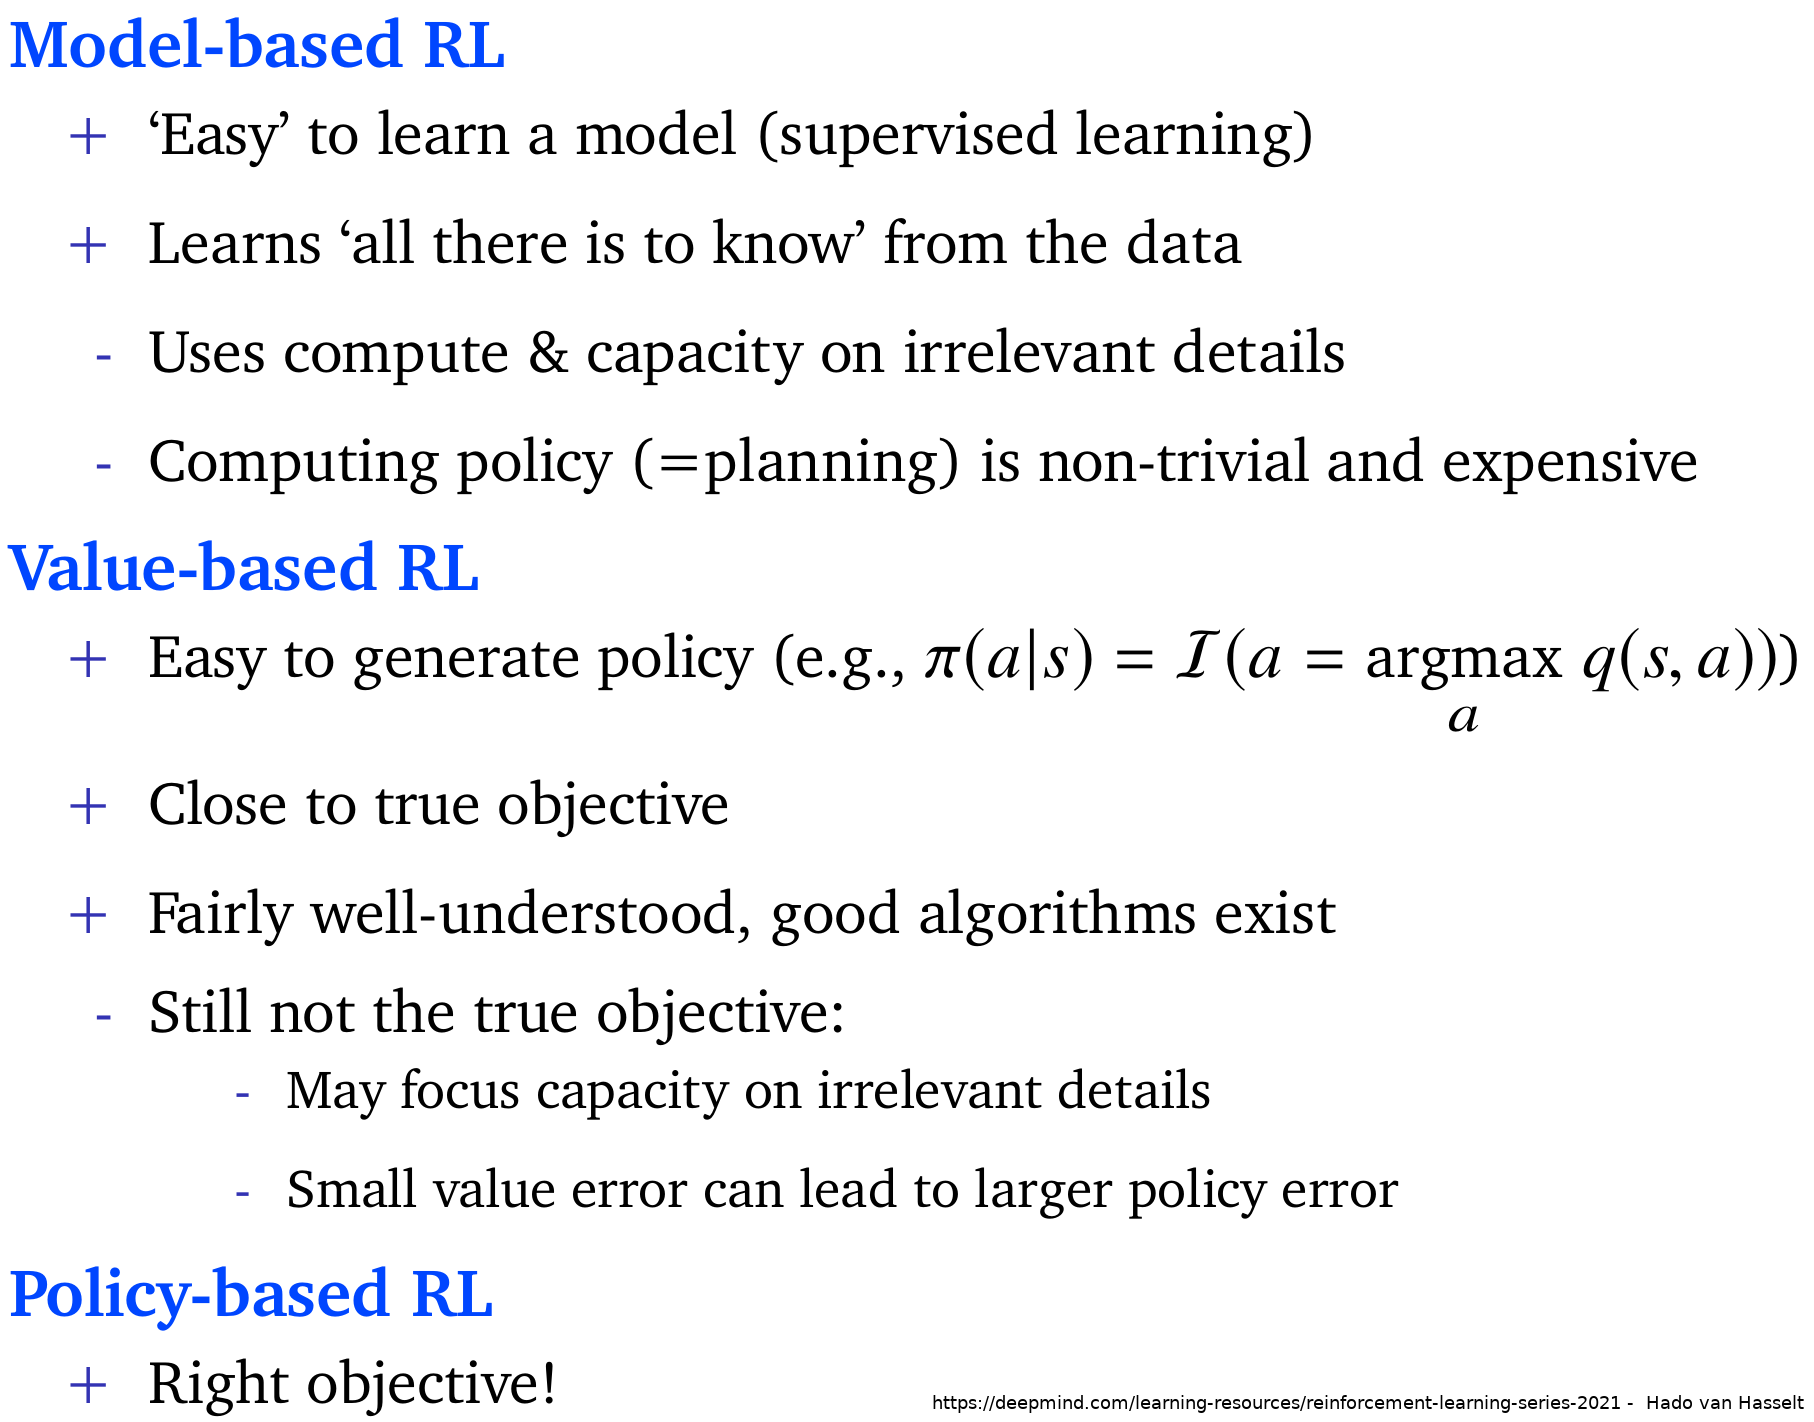
\includegraphics[width=\linewidth]{./images/Lecture9-Policy_gradients_and_actor_critics_deepmind-reinforcement-learning-series-2021.png}
%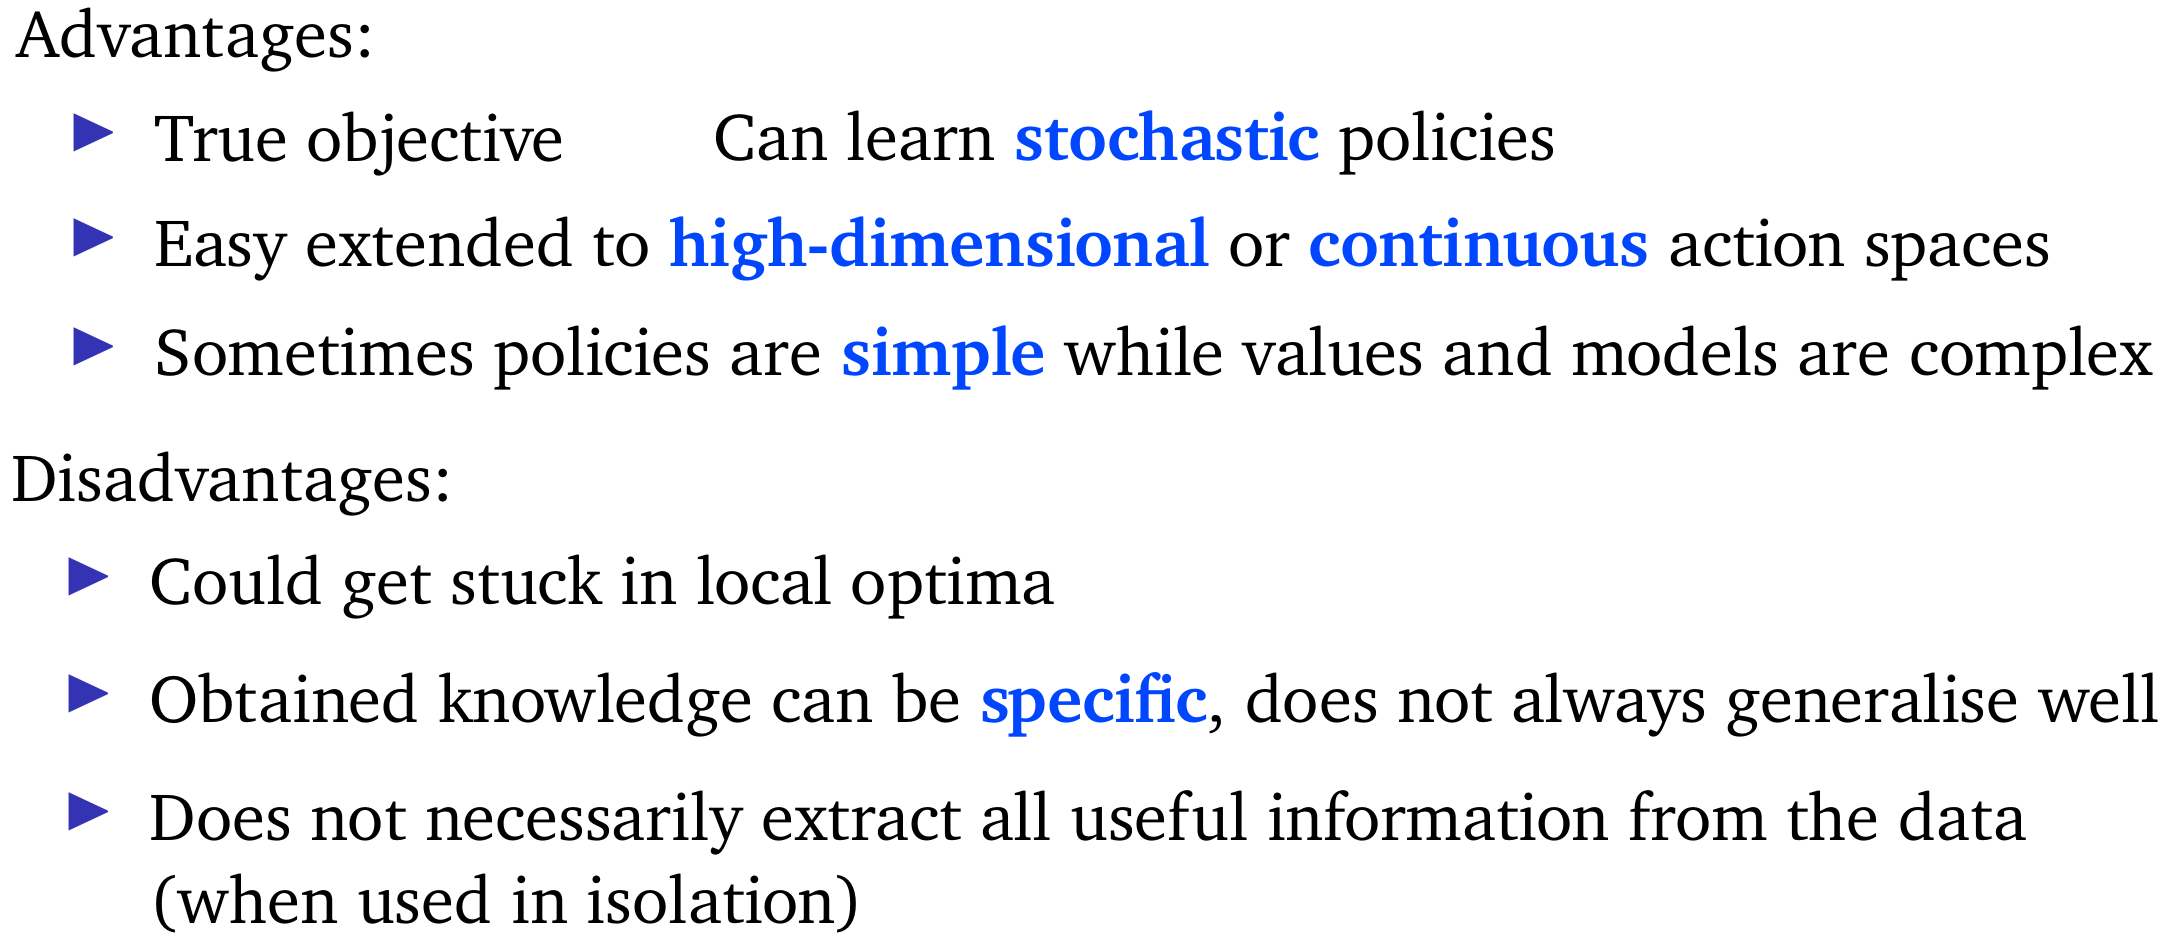
\includegraphics[width=\linewidth]{./images/policy_adv_dis.png}
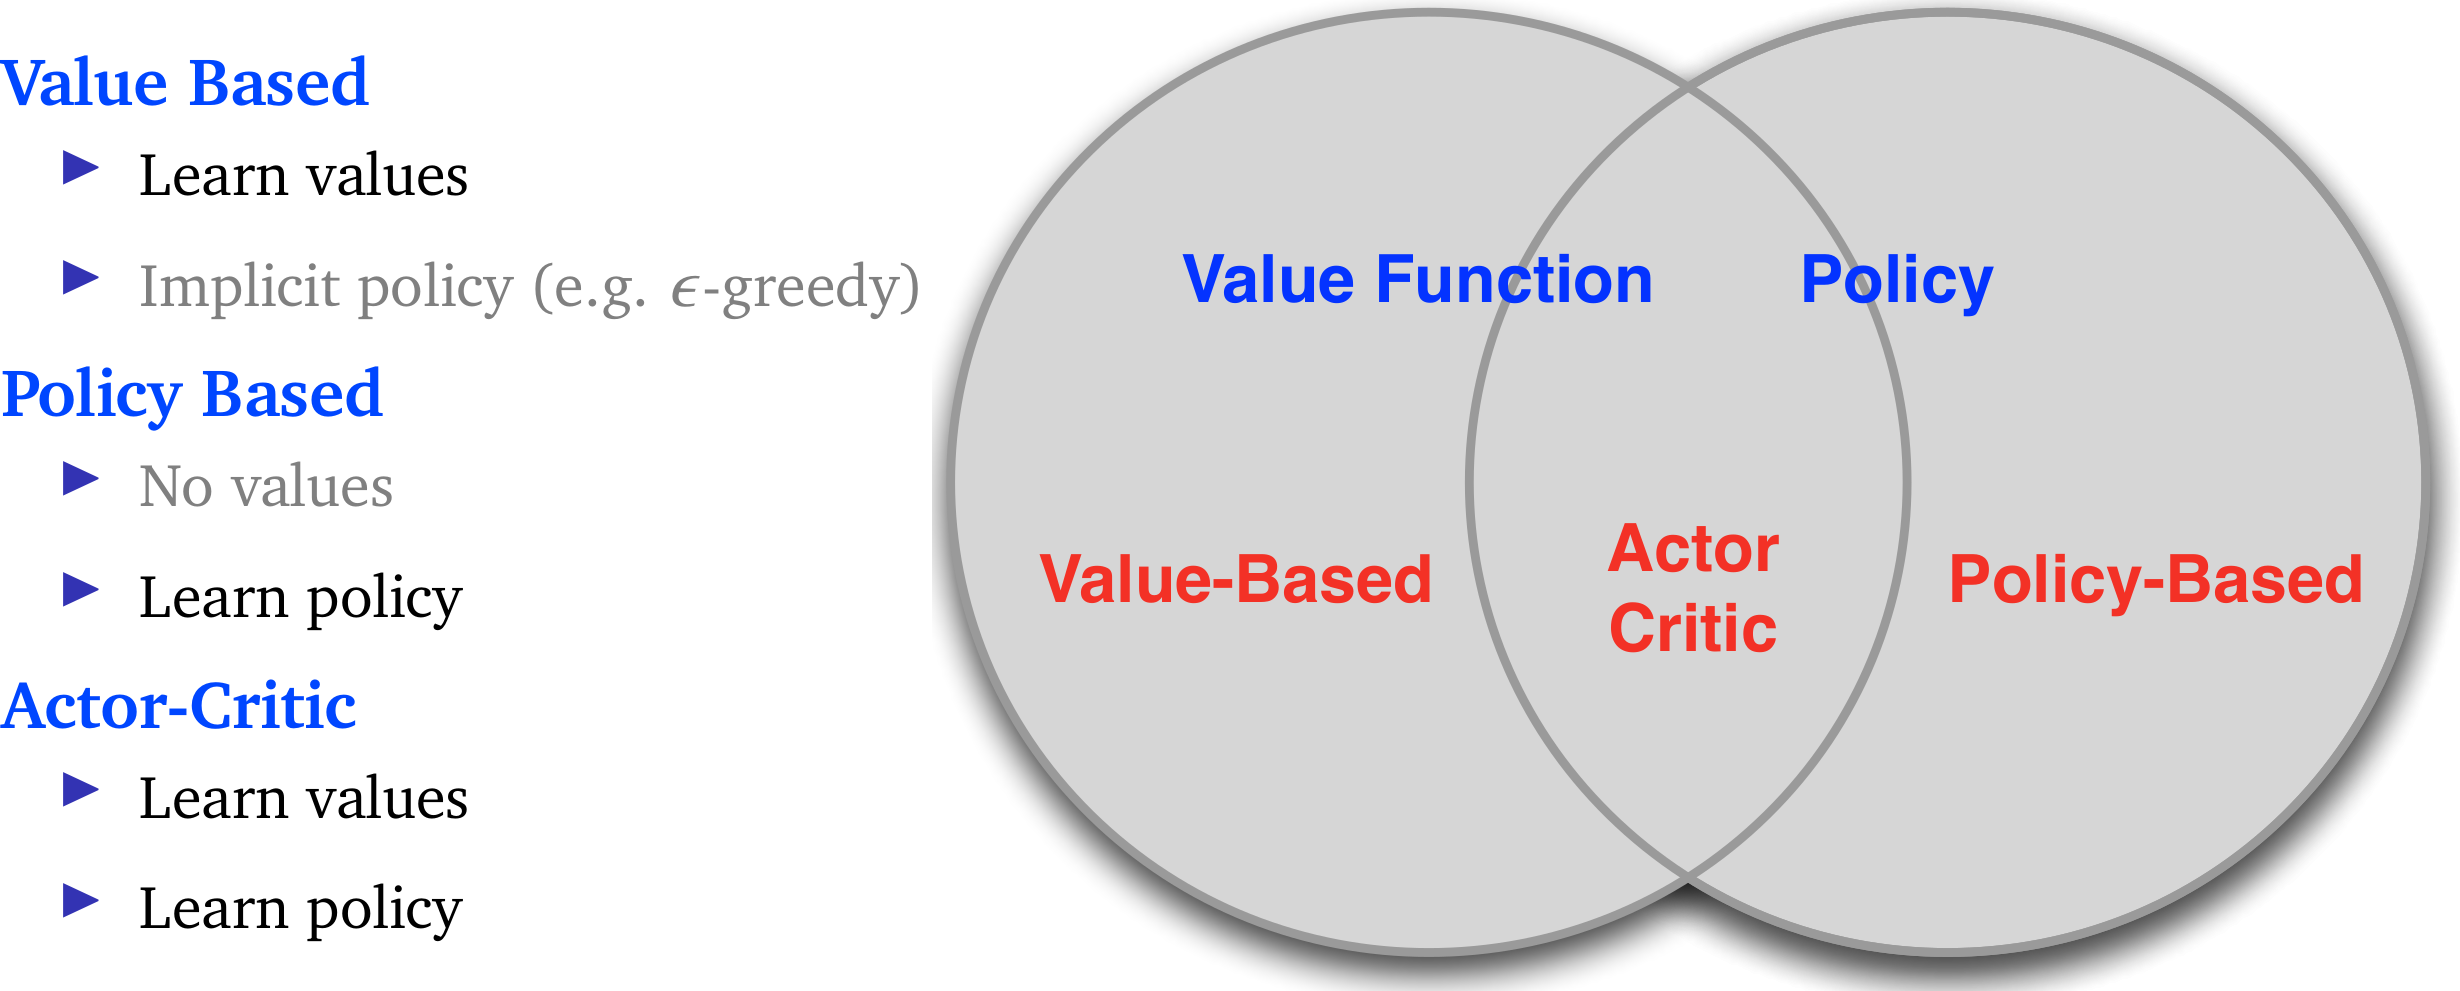
\includegraphics[width=0.9\linewidth]{./images/actorcritics.png}
%\end{figure}FloatBarrier

\vspace{2mm}

\underline{\textbf{Policy learning}}: directly learn $\pi_\theta(s,a)$ minimizing $V(\theta)$:
\begin{align*}
V(s_0,\theta)
&=\mathbb{E}_{\pi_\theta}\left[\sum_{t=0}^T R(s_t,a_t)\right]
=\mathbb{E}_{\pi_\theta}\left[
Q(s_0,\cdot,\theta)
\right]
\\
&=
\sum_{\tau=(s_0,a_0,r_0,\dots,r_{T-1},s_T)}P(\tau;\theta)R(\tau).
\end{align*}
\textbf{Policy Gradient Theorem:} if $\pi_\theta$ differentiable,
$$
\nabla_\theta V(\theta)=\mathbb{E}_{\pi_\theta}\left[
\nabla_\theta\log\pi_\theta(s,\cdot)Q(s_0,\cdot,\theta)
\right].
$$
Its gradient can be approximated as
\begin{align*}
\nabla_\theta V(\theta)
&=\nabla_\theta\sum_{\tau}P(\tau;\theta)R(\tau)=\sum_\tau R(\tau)\nabla_\theta P(\tau;\theta)
\\
&=\sum_\tau
R(\tau)P(\tau;\theta)
\nabla_\theta \log P(\tau;\theta)\\
&\approx \frac{1}{M}\sum_{i=1}^M
R(\tau^i)
\nabla_\theta \log P(\tau^i;\theta)
\\
&=
\frac{1}{M}\sum_{i=1}^M
R(\tau^i)
\left(
\sum_{t=0}^{T-1}\nabla_\theta \log \pi_\theta(a_t|s_t)\right),
\end{align*}
where the last step follows from the fact that
$$
P(\tau^i;\theta)
=
\mu(s_0)\prod_{t=0}^{T-1}\pi_\theta(a_t|s_t)P(s_{t+1}|s_t,a_t).
$$

\textit{Another derivation}: if we exploit the temporal structure, then reward at time $t$ doesnt depend on future timesteps: 
$$\nabla_\theta \mathbb{E}[r_t]=\mathbb{E}\left[
r_t\sum_{r=0}^t\nabla_\theta\log \pi_\theta(a_t|s_t)
\right].
$$
Thus, 
\begin{align*}
\nabla_\theta V(\theta)
%&=
%\mathbb{E}_\tau\left[
%R(\tau)
%\left(
%\sum_{t=0}^{T-1}\nabla_\theta \log \pi_\theta(a_t|s_t)\right)\right]
%\\
%&\approx
%\frac{1}{M}\sum_{i=1}^M
%R(\tau^i)
%\left(
%\sum_{t=0}^{T-1}\nabla_\theta \log \pi_\theta(a_t|s_t)\right)
%\\
%&=
%\frac{1}{M}\sum_{i=1}^M
%\left(
%\sum_{t=0}^{T-1}r_t\right)
%\left(
%\sum_{t=0}^{T-1}\nabla_\theta \log \pi_\theta(a_t|s_t)\right)
%
%
&=
\mathbb{E}_\tau\left[
\sum_{t'=0}^{T-1}r_{t'}
\left(
\sum_{t=0}^{t'}\nabla_\theta \log \pi_\theta(a_t|s_t)\right)\right]
\\
&=
\mathbb{E}_\tau\left[
\sum_{t=0}^{T-1}\nabla_\theta \log \pi_\theta(a_t|s_t)
\sum_{t'=t}^{T-1}r_{t'}
\right]
\\
&\approx
\frac{1}{M}\sum_{i=1}^M\sum_{t=0}^{T-1}\nabla_\theta \log \pi_\theta(a_t^i|s_t^i)
G_{t}^i.
\end{align*}

Note that one can add a baseline to reduce variance:
\begin{align*}
\nabla_\theta V(\theta)
&=
\mathbb{E}_\tau\left[
\sum_{t=0}^{T-1}\nabla_\theta \log \pi_\theta(a_t|s_t)
\left(\sum_{t'=t}^{T-1}r_{t'}-b(s_t)\right)
\right].
\end{align*}
Does not introduce bias. Near optimal choice is the  expected return
$b(s_t)\approx\mathbb{E}[r_t+r_{t+1}+\dots+r_{T-1}]$. 

\textbf{Softmax policy}: $\pi_\theta(s,a)=e^{\phi(s,a)^\top\theta}/\left(\sum\limits_a e^{\phi(s,a)^\top\theta}\right)$. 

\textit{Score function}: $\nabla_\theta\log\pi_\theta(s,a)=\phi(s,a)-\mathbb{E}_{\pi_\pi}[\phi(s,a)].
$
\\[2mm]

\textbf{Gaussian policy}: $\pi_\theta(a(s)\sim\mathcal{N}(\mu_\theta(s), \sigma^2)$. 

\textit{Score function}: $\nabla_\theta\log\pi_\theta(s,a)=
\frac{(a-\mu_\theta(s))}{\sigma^2}\nabla\mu_\theta(s)$

\vspace{2mm}






\vspace{2mm}

\underline{\textbf{Reinforce:}} uses $\Delta\theta_t=\nabla_\theta \log\pi_\theta(s_t,a_t)G_t$
\begin{algorithm}[H]
 \For{each episode $(s_1,a_1,r_1,\dots,s_{T-1},\dots,r_T)\sim\pi_\theta$}{
 \For{$t=1,\dots,T-1$}{
        $\Delta\theta=\alpha\nabla_\theta\log\pi_\theta(a_t|s_t)G_t$
        }
 }
\end{algorithm}

\textbf{Baseline} $b(s)$ to reduce variance:
$$
\theta_{t+1}=\theta_t+\alpha(r_{t+1}-b(s_t))\nabla_\theta\log\pi_\theta(a_t|s_t)$$

\textbf{Actor-Critic}: use $\hat{V}^\pi(s;w)$ (estimated) as baseline

\vspace{2mm}

\underline{\textbf{1-step Actor-Critic:}}
\begin{algorithm}[H]
 \For{$t=1,\dots,T-1$}{
 Sample $a_t\sim\pi_\theta(a|s_t)$, observe $(r_t,s_{t+1})$
 \\
 \scalebox{1}{$\delta_t=r_t+\gamma \hat{V}_w(s_{t+1})-\hat{V}_w(s_t)$\ \ \scalebox{0.9}{(1step TDerror/advantage)}}
 \\ 
 $w\gets w+\beta\delta_t\nabla_w \hat{V}_w(s_t)$ \qquad \quad \ \scalebox{0.9}{(TD(0))}
 \\ 
 $\theta\hspace{0.8mm}\gets\theta\hspace{0.7mm}+\alpha\delta_t\nabla_\theta\log\pi_\theta(a_t|s_t)$
 \ \ \ \scalebox{0.9}{(policy gradient)}
        }
\end{algorithm}

\vspace{1mm}

\textbf{Increasing stability} (TRPO,PPO): add KL regularization to 
\scalebox{1}{an older policy $\pi_{\textrm{old}}$:
do policy gradient with $J(\theta)-\eta\textrm{KL}(\pi_{\textrm{old}},\pi_\theta)$:}
 $$
 \textrm{KL}(\pi_{\textrm{old}}\|\pi_\theta)=\mathbb{E}_s\left[\int_A\pi_{\textrm{old}}(a|s)
\log\frac{\pi_{\textrm{old}}(a|s)}{\pi_\theta(a|s)}
\textrm{d}a\right]
$$

\newpage
\FloatBarrier

%---------------------------------------------------------------------------

%\rule{0.3\linewidth}{0.25pt} \\
%Copyright \copyright\ 2018 Francesco Saverio Zuppichini
%
%\scriptsize
%
%\href{https://github.com/FrancescoSaverioZuppichini/Reinforcement-Learning-Cheat-Sheet}{https://github.com/FrancescoSaverioZuppichini/Reinforcement-Learning-Cheat-Sheet}

\end{multicols}

%\newpage
%
%\begin{multicols}{3}
%
%\section{Double Deep Q Learning}
%
%\end{multicols}

\end{document}
